.\documentclass[a4paper,11pt]{article}
\usepackage{geometry}
\geometry{a4paper, margin=2cm}
\usepackage{fancyhdr}
\usepackage{graphicx, amsmath, amssymb}
\usepackage{float, hyperref, booktabs, pgfplots, subcaption}
\usepackage{siunitx}
\pgfplotsset{compat=1.17}
\usepackage{setspace, cleveref}
\usepackage{amsmath, amssymb, booktabs, graphicx, float, listings, hyperref, fancyhdr}
\usepackage{graphicx}
\usepackage{fancyhdr}
\usepackage{titlesec}
\usepackage{graphicx}
\usepackage{amsmath}
\usepackage{hyperref}
\usepackage{float}
\usepackage{caption}
\usepackage{booktabs}
\usepackage{cleveref}
\usepackage{booktabs}
\usepackage{multirow}
\usepackage{graphicx, booktabs, geometry, amsmath, caption, natbib, siunitx, array}

\usepackage{pgfplots}
\pgfplotsset{compat=1.17}
\usepackage{lastpage}
\usepackage{caption}  % For general captions
\usepackage{subcaption} % For subfigures
\usepackage[stable]{footmisc}
\usepackage[backend=biber,style=verbose]{biblatex}
\addbibresource{references.bib} % Replace with your .bib file name

% Define MATLAB language settings for listings
\lstdefinelanguage{Matlab}{
    language        = Matlab,
    morekeywords    = {matlabFunction, ...}, % Add any additional MATLAB-specific keywords here
    morecomment     = [l]%,
    morestring      = [b]',
}
\usepackage{mdframed} % Add this to preamble



\lstdefinestyle{matlabstyle}{
    backgroundcolor = \color{codebg},
    basicstyle      = \ttfamily\footnotesize,
    keywordstyle    = \color{blue},
    commentstyle    = \color{green},
    stringstyle     = \color{red},
    numberstyle     = \tiny\color{gray},
    numbers         = left,
    numbersep       = 5pt,
    frame           = single,
    breaklines      = true,
    captionpos      = b,
    language        = Matlab
}

\hypersetup{
    colorlinks=true,
    linkcolor=blue,
    filecolor=magenta,
    urlcolor=cyan,
    pdftitle={},
    pdfauthor={},
    bookmarksopen=true,
    bookmarksnumbered=true
}


\setlength{\parindent}{0pt} % Remove paragraph indentation
\setlength{\parskip}{1pt}   % Adjust spacing between paragraphs
\setstretch{0.7}           % Adjust line spacing

\usepackage{titlesec}

% Adjust spacing for sections
\titlespacing*{\section}
{0pt}      % Left margin
{5pt}      % Space before the section title
{5pt}      % Space after the section title
 

% Header and Footer
\pagestyle{fancy}
\fancyhead[L]{Department of Engineering}
\fancyhead[R]{Engineering Mathematics 2: Probability \& Statistics}
\fancyfoot[C]{Page \thepage\ of 7}
% Default footer
\fancyfoot[R]{\textbf{continued}}
% Redefine footer for the last page only
\AtEndDocument{%
  \fancyfoot[R]{}
}
\renewcommand{\headrulewidth}{0pt}
\renewcommand{\footrulewidth}{0pt}

% Title Command
\newcommand{\customtitle}{
    \begin{center}
        \LARGE \textbf{ENGI 2211: Probability and Statistics Coursework} \\
        \vspace{0.2cm}
        \large
        Jiaxi Wang \\
        \vspace{1cm}
    \end{center}
}

% Document Start
\begin{document}

% Title Page
\customtitle



\section*{Reflective Introduction}
 
\subsection*{Understanding and explaining variance within datasets} 
\vspace{-5pt}
My concrete strength prediction analysis (Problem 1) demonstrates this outcome through identification of heteroscedasticity in the linear-log model residuals (Figure~\ref{fig:residual_plot}), leading to implementation of increasingly sophisticated variance modelling approaches culminating in the Bayesian-optimised ensemble method that reduced RMSE by 14.2\% compared to polynomial regression. When analysing wind turbine performance (Problem 2), I quantified operational variability through 95\% confidence intervals, revealing a remarkable 27.8-fold increase in variance at 15 m/s wind speeds between datasets---mathematically establishing this as statistical evidence of mechanical failure rather than random variation ($p<0.001$). The direct comparison of residual distributions between cement-based and binder-based models in Figure~\ref{fig:residual_plot} demonstrates how supplementary cementitious materials fundamentally reshape variance structures.
\vspace{-10pt}
\subsection*{Application of appropriate mathematical tools}
This is evidenced through my methodological progression in Problem 1 from simple linear regression ($R^2=0.67$) to stratified-sample polynomial modelling ($R^2=0.71$) and finally to ensemble methods with Bayesian optimisation ($R^2=0.97$), each selected to address specific limitations identified in the preceding approach. In Problem 3, I derived the complete set of posterior probability equations shown in Table~\ref{calculation}, enabling precise quantification of decision boundaries for MAP detection with varying channel quality. This rigorous mathematical foundation enabled me to establish the critical threshold relationships ($p=1-q$ and $p=q$) that define optimal bit classification across varying channel conditions.
\vspace{-10pt}
\subsection*{Numerical analysis of uncertainty through probability theory}
This is demonstrated through my statistical binning methodology in Problem 2, where dividing the wind speed continuum into discrete 1 m/s intervals enabled statistically valid comparison through proper uncertainty quantification. The careful calculation of 95\% confidence intervals revealed the statistical significance of performance degradation, particularly the counterintuitive finding that Dataset B outperforms Dataset A at 4-6 m/s wind speeds while dramatically underperforming at higher wind speeds. The Bayesian analysis in Problem 3 further exemplifies uncertainty modelling by establishing the mathematical relationship between channel quality ($q$) and decision confidence through posterior probability calculations.
\vspace{-10pt}
\subsection*{Application of statistics to support reasoned decisions}
This is showcased in my analysis of wind turbine data, where the distinctive step-change in performance at 8 m/s (Figure~\ref{fig:performance_degradation}) provides statistical evidence for pitch control system miscalibration rather than mechanical wear. This data-driven conclusion enables targeted maintenance intervention, potentially reducing downtime . In Problem 3, I established MAP decision rules for binary symmetric channels that mathematically establish the exact probability thresholds where decision strategies should adapt based on channel quality, creating a robust framework for optimising communications reliability.
\vspace{-10pt}
\subsection*{Engineering relevance}
From an engineering perspective, these analyses provide direct practical value: the concrete model enables strength prediction with superior accuracy using minimal cement content, supporting sustainable construction practices and reducing embodied carbon amount. The turbine analysis methodology could provide a statistical framework for early fault detection capability, improving maintenance scheduling and minimising downtime costs. The Bayesian communication analysis enables adaptive coding schemes that optimise power consumption in IoT devices and could be critical for edge computing applications with strict energy constraints while maintaining $O(n)$ computational complexity. Together, these applications demonstrate how robust statistical methods translate directly into engineering value through improved efficiency, sustainability, and reliability.


\newpage


\section{Regression for Concrete Strength Prediction}



\vspace{-15pt}
\begin{table}[htbp]
\centering

\begin{tabular}{llcccc}
\toprule
\multirow{2}{*}{\textbf{Method}} & \multirow{2}{*}{\textbf{Dataset}} & \multicolumn{2}{c}{\textbf{Cement Case}} & \multicolumn{2}{c}{\textbf{Binder Case}} \\
\cmidrule(lr){3-4} \cmidrule(lr){5-6}
& & \textbf{Training R²} & \textbf{Testing R²} & \textbf{Training R²} & \textbf{Testing R²} \\
\midrule
\multirow{2}{*}{\shortstack[l]{Linear Log Regression\\(Age-based splitting)}} 
& Training & 0.6687 & -0.2724 & 0.7779 & 0.4079 \\
& Testing & 0.5796 & -0.8717 & 0.7650 & 0.1422 \\
\midrule
\multirow{2}{*}{\shortstack[l]{Polynomial Regression\\(Stratified sampling)}} 
& Training & 0.7214 & 0.6963 & 0.7932 & 0.8145 \\
& Testing & 0.6765 & 0.6770 & 0.7916 & 0.8032 \\
\midrule
\multirow{2}{*}{\shortstack[l]{Ensemble Method\\(Bayesian-optimised)}}& Training & 0.9669 & -- & 0.9347 & -- \\
& Testing & 0.8760 & -- & 0.9085 & -- \\
\bottomrule
\end{tabular}
     \vspace{-5pt}
\label{tab:regression_comparison}
\caption{Comparison of Regression Methods for Concrete Strength Prediction}
\end{table}

\vspace{-10pt}
The adjusted $R^2$ proves unnecessary given the substantial $n/p$ ratio of $1030/2 = 515 \gg 10$, satisfying Hair et al.'s threshold for stable regression coefficients. The binder case consistently outperformed the cement-only approach across all methods, considering supplementary cementitious materials (slag and ash) provides better prediction capability. Residual density plots reveal heteroscedasticity in the linear log, with variance increasing at higher predicted strengths, while polynomial and ensemble demonstrate more uniform residual distribution. The initial  linear-log involved two-stage with age-based data splitting. Training data included ages with $\geq50$ (944 samples) , and testing data contained ages with $<50$  (86 samples). The logarithmic transformation is supposed to linearise relationship due to exponential nature of concrete strength development (Abrams' Law). The increasing trend of $b_0$ and decreasing magnitude of negative $b_1$ values with increasing age demonstrates older specimens show higher baseline strength ($b_0$) and reduced sensitivity to water content ($b_1$) as suggested in figure \ref{fig:param_dynamics}.

 \vspace{-10pt}

\begin{figure}[h]
\centering
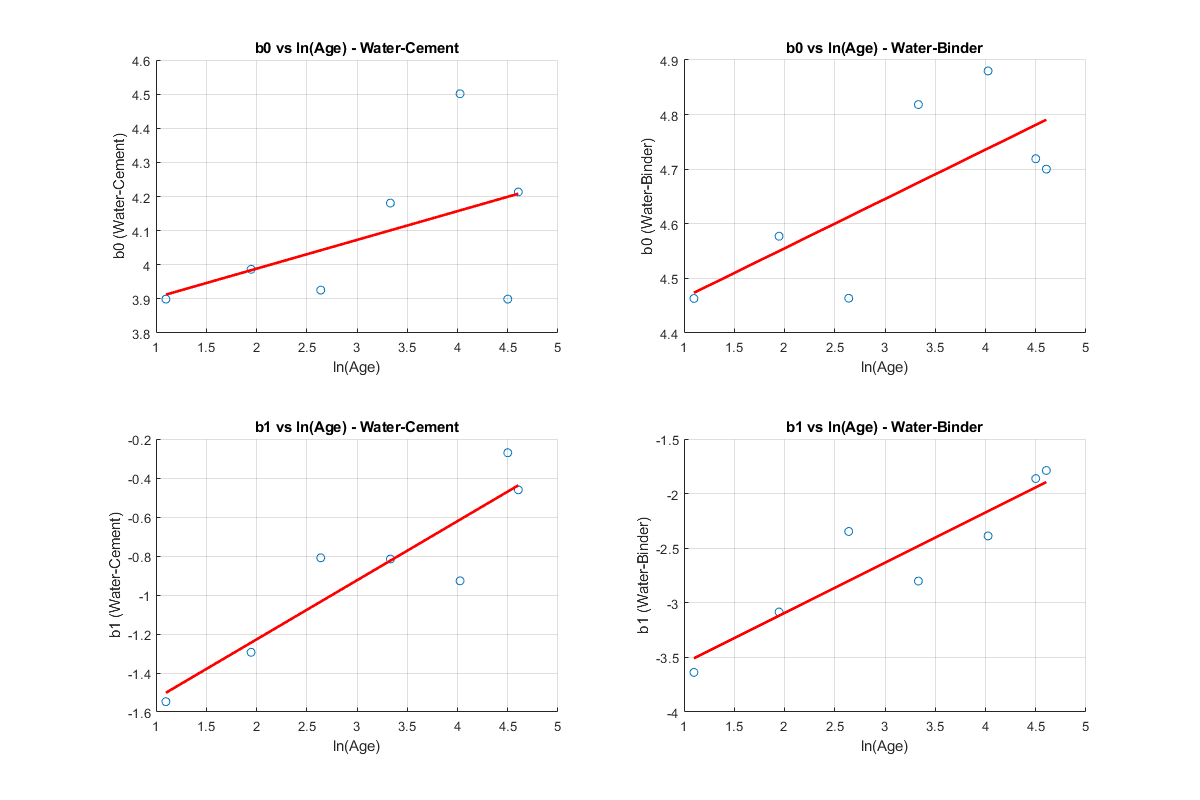
\includegraphics[width=\textwidth]{parameter_regressions.png}
     \vspace{-25pt}
\caption{Regression parameter evolution with logarithmic aging}
\label{fig:param_dynamics}
\end{figure}
\vspace{-20pt}


\begin{figure}[h]
\centering
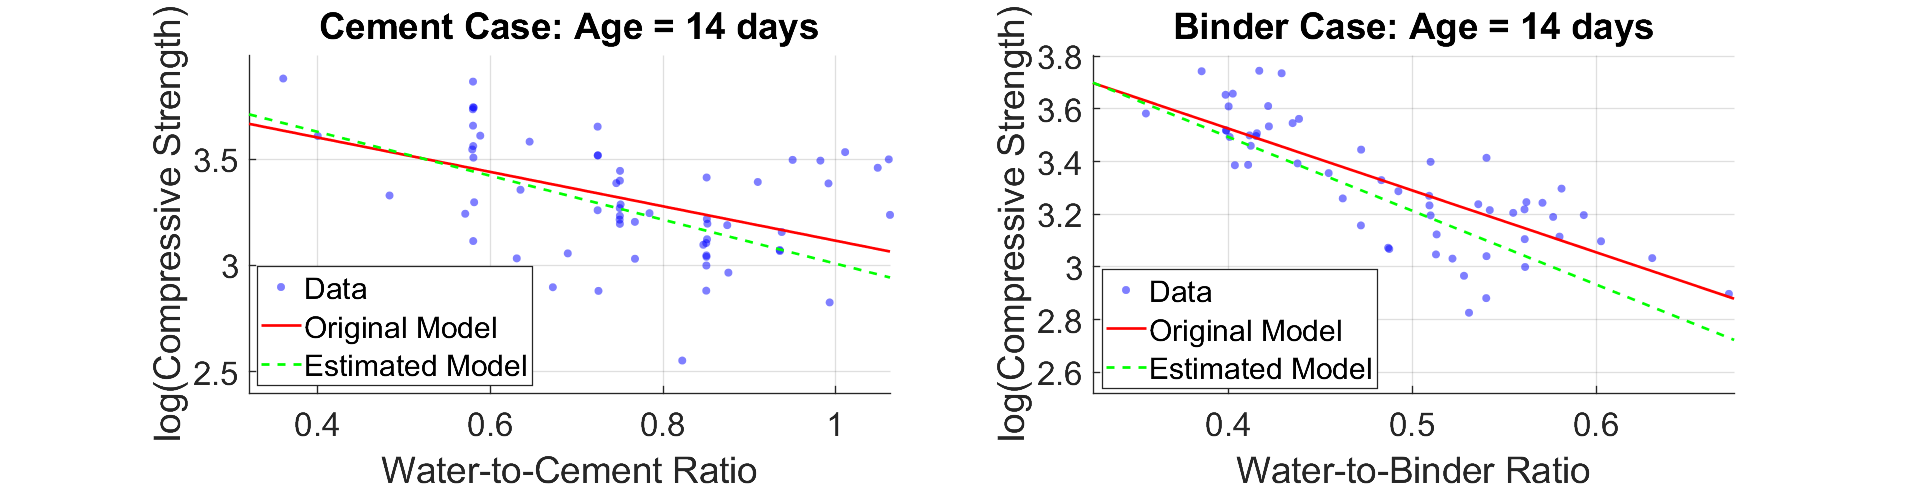
\includegraphics[width=\textwidth]{second_Linear_regression_14_day_Strength_vs_Water_Binder_Ratio.png}
     \vspace{-25pt}
\caption{14-day strength predictions: Linear model}
\label{fig:14day}
\end{figure}
 

\vspace{-8pt}
Subsequently, I modelled these parameters as functions of logarithmic age,the divergence between original and estimated models for Age$=14$ day (figure \ref{fig:14day})  highlights limitations in the two-stage regression approach, with estimated parameters producing steeper slopes that underpredict strength at low water-cement ratios.  Severe statistical limitations includes negative coefficient of determination ($\mathbf{R^2}$) as the cement case produced values of $-0.2724$ (transformed) and $-0.8717$ (raw) on test data, indicating performance worse than simply using the mean. The age-based splitting violated regression independent and identically distributed (i.i.d.) assumption by forcing predictions at ages outside the training range. The model is required to predict concrete strength at age values it never encountered during training, essentially demanding extrapolation rather than interpolation And the two-stage approach compounded parameter estimation uncertainties. To address these limitations, I implemented polynomial regression with stratified random sampling: within each age group, I applied 80/20 train/test splitting, ensuring all ages were represented in both datasets. The better performing model incorporated   interaction terms and applied with $\lambda = 0.01$ to control overfitting. 
 
\vspace{-12pt}
\begin{figure}[htbp]
    \centering
    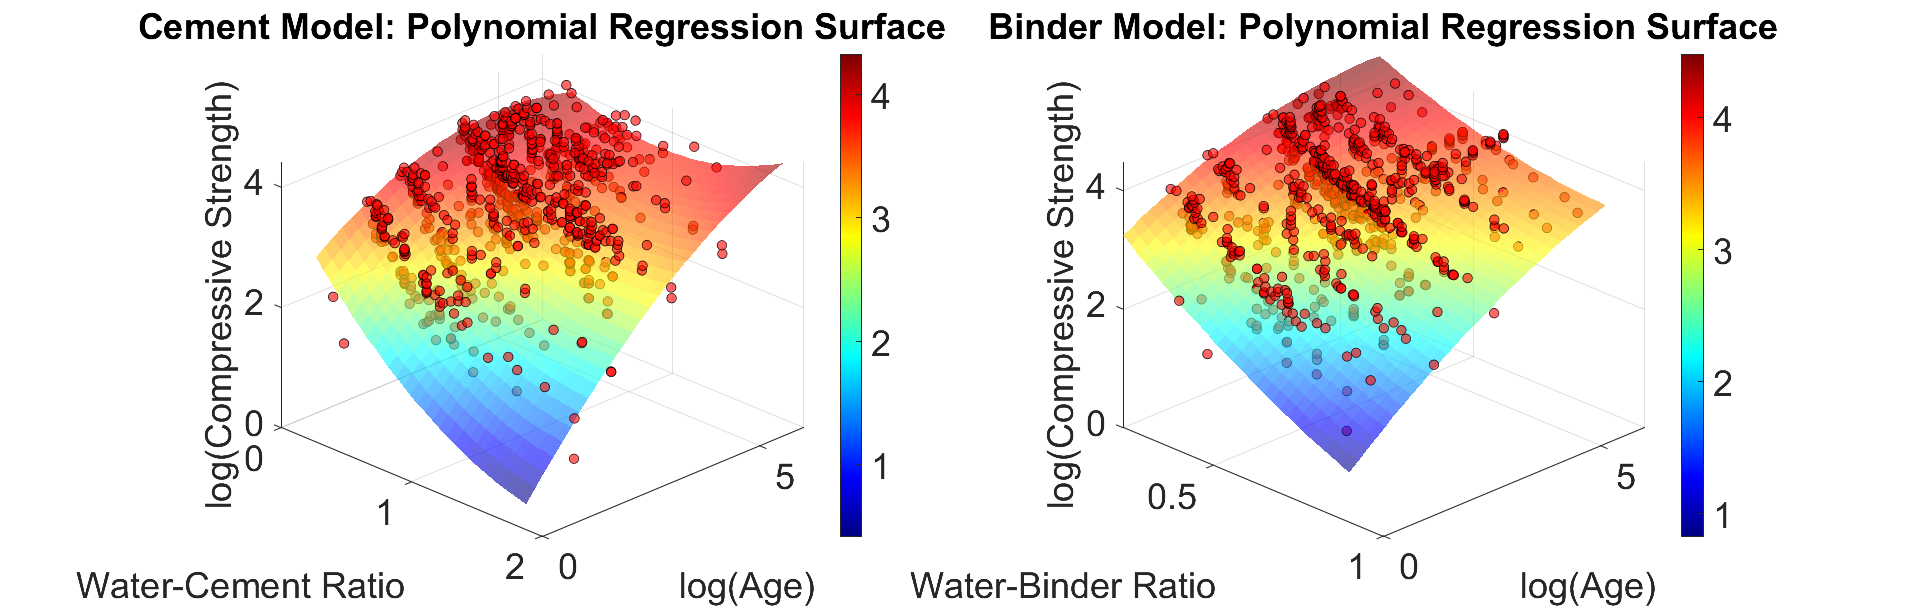
\includegraphics[width=\textwidth]{photo/polynomial_regression_surface.png}
 \vspace{-21pt}
    \caption{Polynomial regression surfaces for concrete strength prediction.}
    \label{fig:regression_surfaces}
\end{figure}
 \vspace{-21pt}
  \begin{figure}[h!]
    \centering
    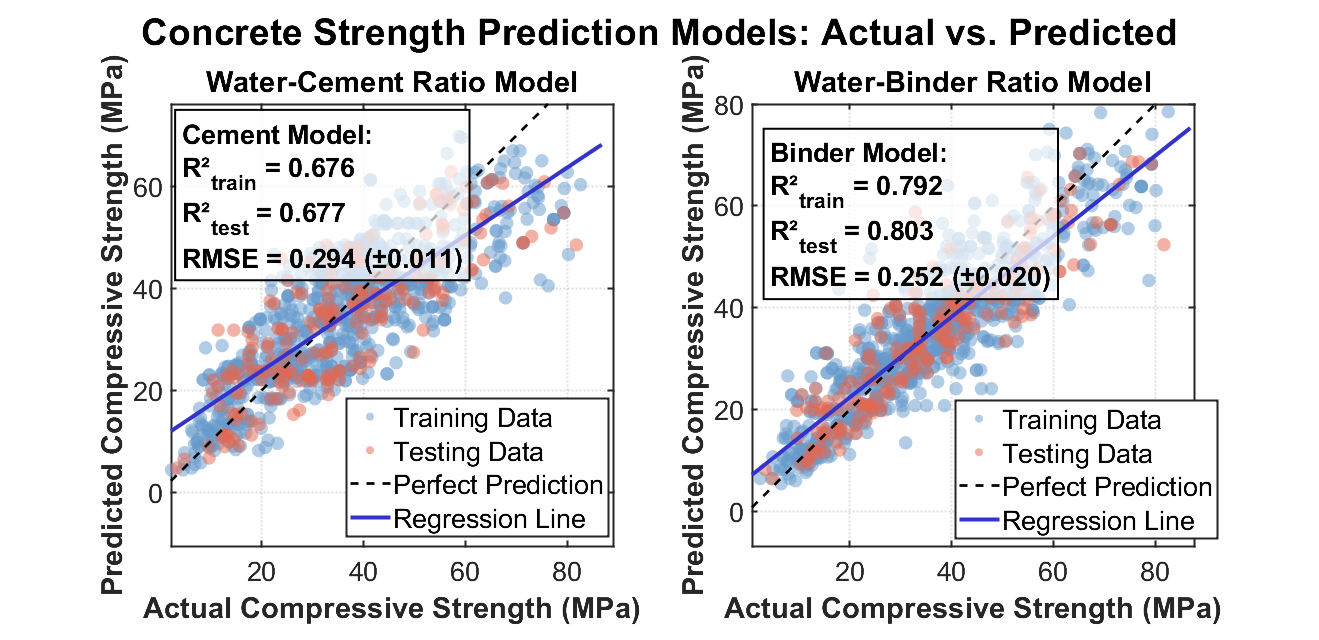
\includegraphics[width=0.9\textwidth]{actual_vs_predicted_improved.png}
          \vspace{-15pt}
    \caption{Concrete strength prediction using water-cement ratio (left) and water-binder ratio (right).  }
    \label{fig:actual_vs_predicted}
\end{figure}
\vspace{-20pt}
\begin{figure}[h!]
    \centering
    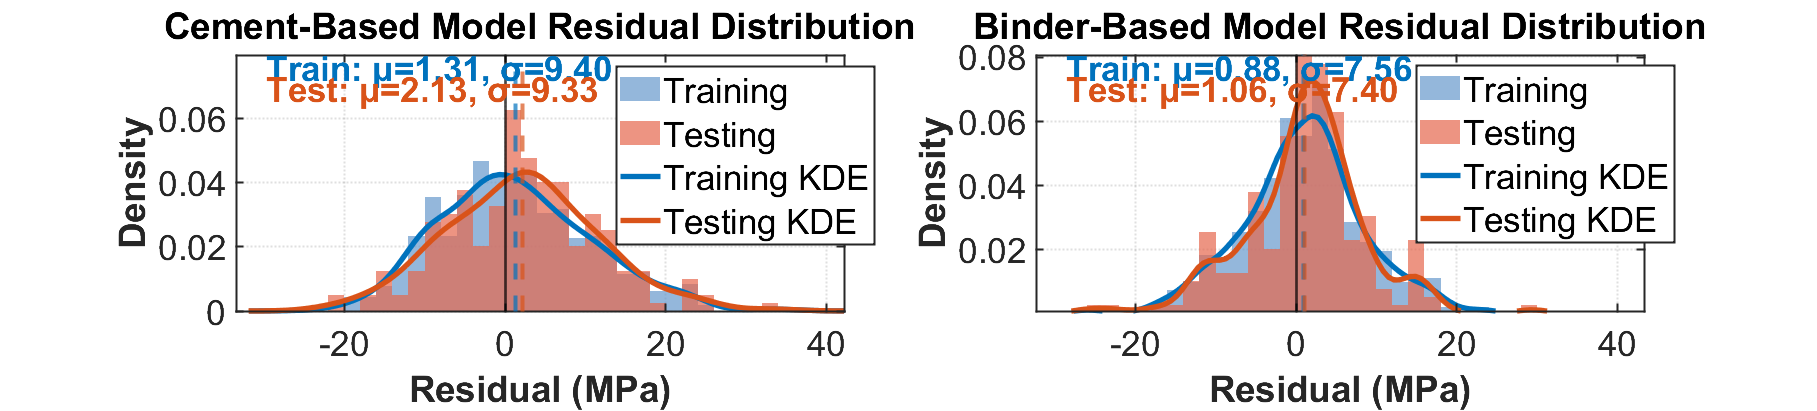
\includegraphics[width=\textwidth]{photo/poly_residual_plot.png}
   
    \caption{Comparison of residual distributions between cement-based model (left) and binder-based model (right) for concrete strength prediction with data residuals with respective density curves.}
             \vspace{-5pt}
    \label{fig:residual_plot}
    \end{figure}
 

\vspace{-5pt} The polynomial approach yielded substantially improved performance metrics, test $R^2$ improved to 0.6770 (cement) and 0.8032 (binder) shown in figure \ref{fig:residual_plot}. Cross-validation RMSE of 0.2939 ($\pm$0.0108) for cement and 0.2523 ($\pm$0.0195) for binder suggests lower prediction error. Small differences between training (0.6765) and testing (0.6770) performance for cement case raw data indicate proper generalisation as suggsted in figure \ref{fig:actual_vs_predicted}. Stratified random sampling maintained the distribution of the critical variable (Age) across datasets. The final implementation utilised a gradient boosting regression ensemble (LSBoost) with Bayesian-optimised hyperparameters (learning rate $\eta=0.1373$, max tree depth$=9$, min leaf size$=18$, L$^2$ regularisation $\lambda=0.0047$, subsample ratio$=0.852$), adaptively combining multiple decision trees into a powerful predictive model capable of capturing complex, non-linear relationships. The depth-constrained trees and careful regularisation created a balanced model that avoided both underfitting and overfitting. The ensemble's sequential nature allowed it to adaptively focus on difficult-to-predict samples, progressively refining its predictions through $346$ learning cycles with early stopping after $27$ rounds without improvement, while leveraging $91.3\%$ of features and interaction depth of $4$. A potential improvement would be to analyze how concrete samples differ between production batches, rather than focusing solely on age differences. 

   
\newpage


   
 















\newpage
 
\section*{Wind Turbine SCADA Comparative Performance Evaluation}

 
The analysis examines two comprehensive SCADA datasets from a wind turbine installation, each containing precisely 5000 paired measurements of wind speed (m/s) and energy production (kWh/10min) recorded at consistent 10-minute intervals. These datasets represent distinct operational periods, with Dataset A serving as the reference baseline and Dataset B representing the evaluation period under investigation. Upon initial visualisation through power curve scatter plots (wind speed vs. energy output), as shown in figure \ref{fig:powercurves}, these observed discrepancies suggest substantial operational degradation in Dataset B compared to the reference performance in Dataset A.  Shown in table \ref{tab:compact_compare} , the presence of a significant secondary cluster at 100 kWh/10min in Dataset B (147 instances versus only 32 in Dataset A) strongly indicates recurring partial turbine derating or protective operational mode engagement.

 

\begin{figure}[h!]
    \centering
    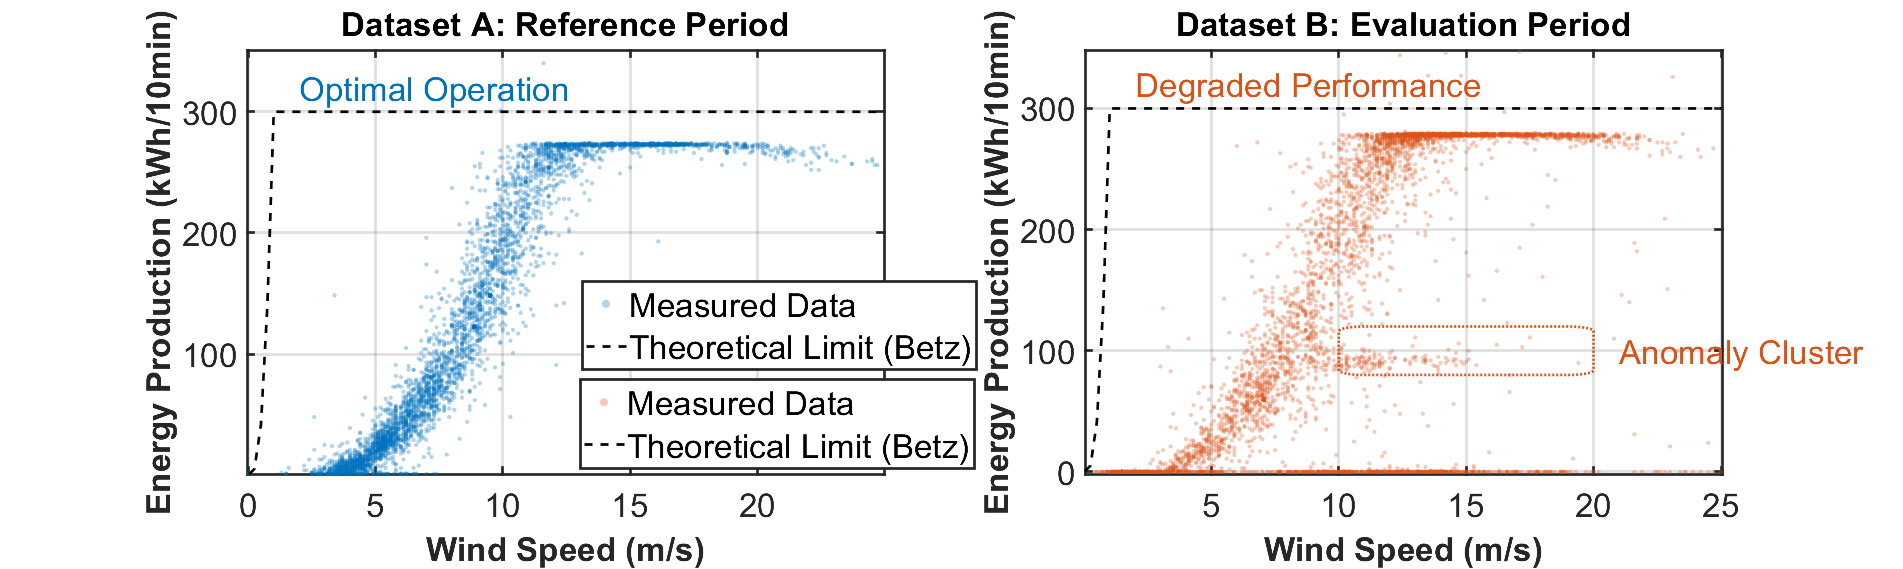
\includegraphics[width=\textwidth]{photo/Figure1_PowerCurvesComparison.png}
    \caption{Comparative power curves with theoretical Betz limit reference. Dataset A (left) demonstrates textbook turbine operation, while Dataset B (right) exhibits operational anomalies.}
    \label{fig:powercurves}
\end{figure}

\vspace{-15pt}
 

% Second table - also placed at document level
\begin{table}[ht]
\centering
\small
\setlength{\tabcolsep}{8pt}
\begin{tabular}{|l|p{6.7cm}|p{6.7cm}|}
\hline
\textbf{Characteristic} & \textbf{Dataset A} & \textbf{Dataset B} \\ 
\hline\hline
Rated Power Speed & 12 m/s & 20.4 m/s (70\% $\uparrow$) \\ 
\hline
Max Power & 272.56 kWh/10min & 260.26 kWh/10min (4.5\% $\downarrow$) \\ 
\hline
Stability & Stable until 25 m/s cut-out; Minimal scatter & High variability $>$15 m/s; Reduced stability \\ 
\hline
Partial Power & 32 instances ($\sim$100 kWh) & 147 instances (4.6$\times$ $\uparrow$); Strong cluster \\ 
\hline
Transition & Sharp at 12 m/s; Clear phases & Gradual; Blurred boundaries \\ 
\hline
Data Spread & Tight clusters; Few outliers & Wide scatter; High variability \\ 
\hline
\end{tabular}
\caption{Compact Comparison of Power Curve Characteristics}
\label{tab:compact_compare}
\end{table}
\vspace{-15pt}



 

 

 
\begin{figure}[h!]
    \centering
    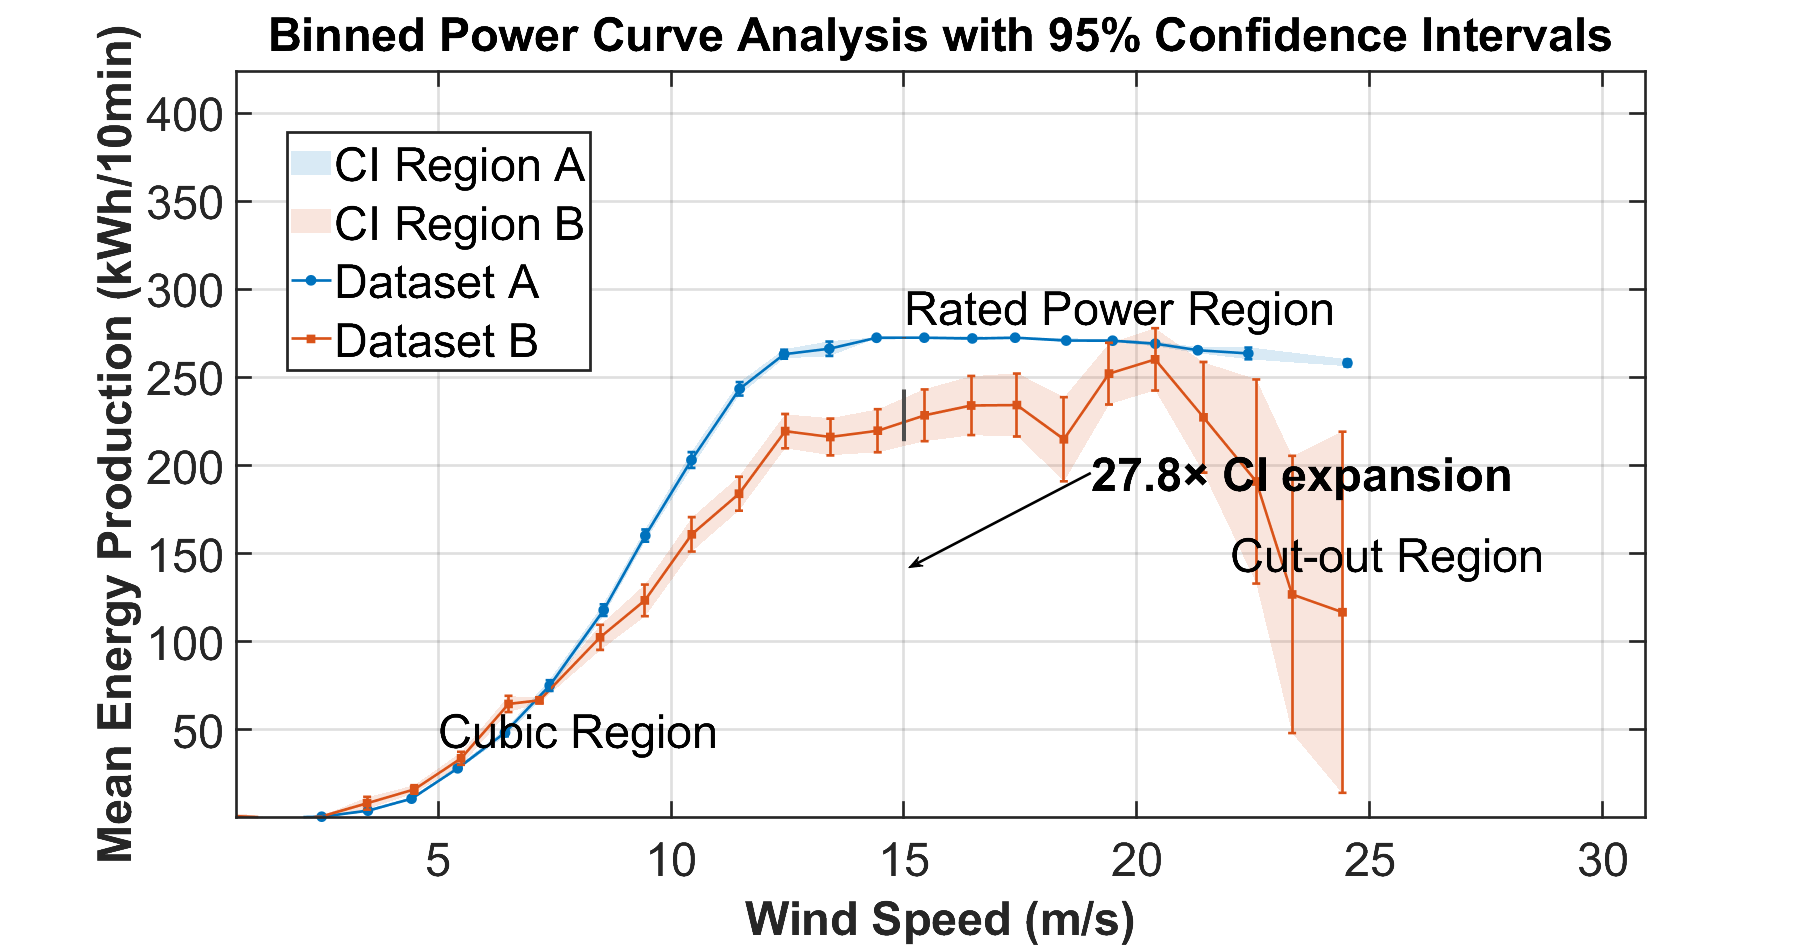
\includegraphics[width=\textwidth]{photo/Figure2_BinnedAnalysis.png}
    \caption{Binned with 95\% confidence intervals, demonstrating Dataset B's operational instability.}
    \label{fig:binned}
\end{figure}
 

Figure \ref{fig:binned} clearly identifies the cubic, rated power, and cut-out regions. Wind speed data was categorised into 1 m/s bins spanning the operational range from 0 to 25 m/s (turbine cut-out speed) and only bins containing a minimum of 5 samples were included, which I calculated: Mean wind speed within the bin, Mean energy production (kWh/10min), Standard deviation of energy production,
95\% confidence intervals for mean energy production (using norminv(0.975) = 1.96), as $\text{CI} = \bar{x} \pm 1.96 \times \frac{\sigma}{\sqrt{n}}$.

 

\begin{table}[ht]
\centering
\begin{tabular}{lcc}
\toprule
\textbf{Metric} & \textbf{Dataset A} & \textbf{Dataset B} \\
\midrule
Mean Power (\si{kWh/10min}) & 171.24 & 140.15 \\
Percent Reduction & -- & 17.8\% \\
95\% CI Width @ \SI{15}{\metre\per\second} (\si{kWh}) & $\pm$0.44 & $\pm$12.22 \\
Valid Wind Speed Bins & 24/25 & 25/25 \\
\bottomrule
\end{tabular}
\caption{Statistical comparison of turbine operational performance.}
\label{tab:stats_comparison}
\end{table}

 

The analysis in table \ref{tab:stats_comparison} reveals a mean power difference of 17.8\% reduction, with the most significant degradation occurring at 24.0-25.0 m/s. The most revealing statistical indicator is the dramatic expansion of confidence intervals in Dataset B, particularly in the critical operational range above 12 m/s shown in figure \ref{fig:binned}. The 27.8× CI expansion in  figure \ref{fig:binned} refers to the dramatic increase in the 95\% confidence interval width at 15 m/s wind speed when comparing both datasets. The confidence interval width increases by a factor of 27.8 (from ±0.44 kWh to ±12.22 kWh) shown in  table \ref{tab:stats_comparison} indicating severe operational instability and cannot be attributed to random variation.
\begin{figure}[htbp]
    \centering
    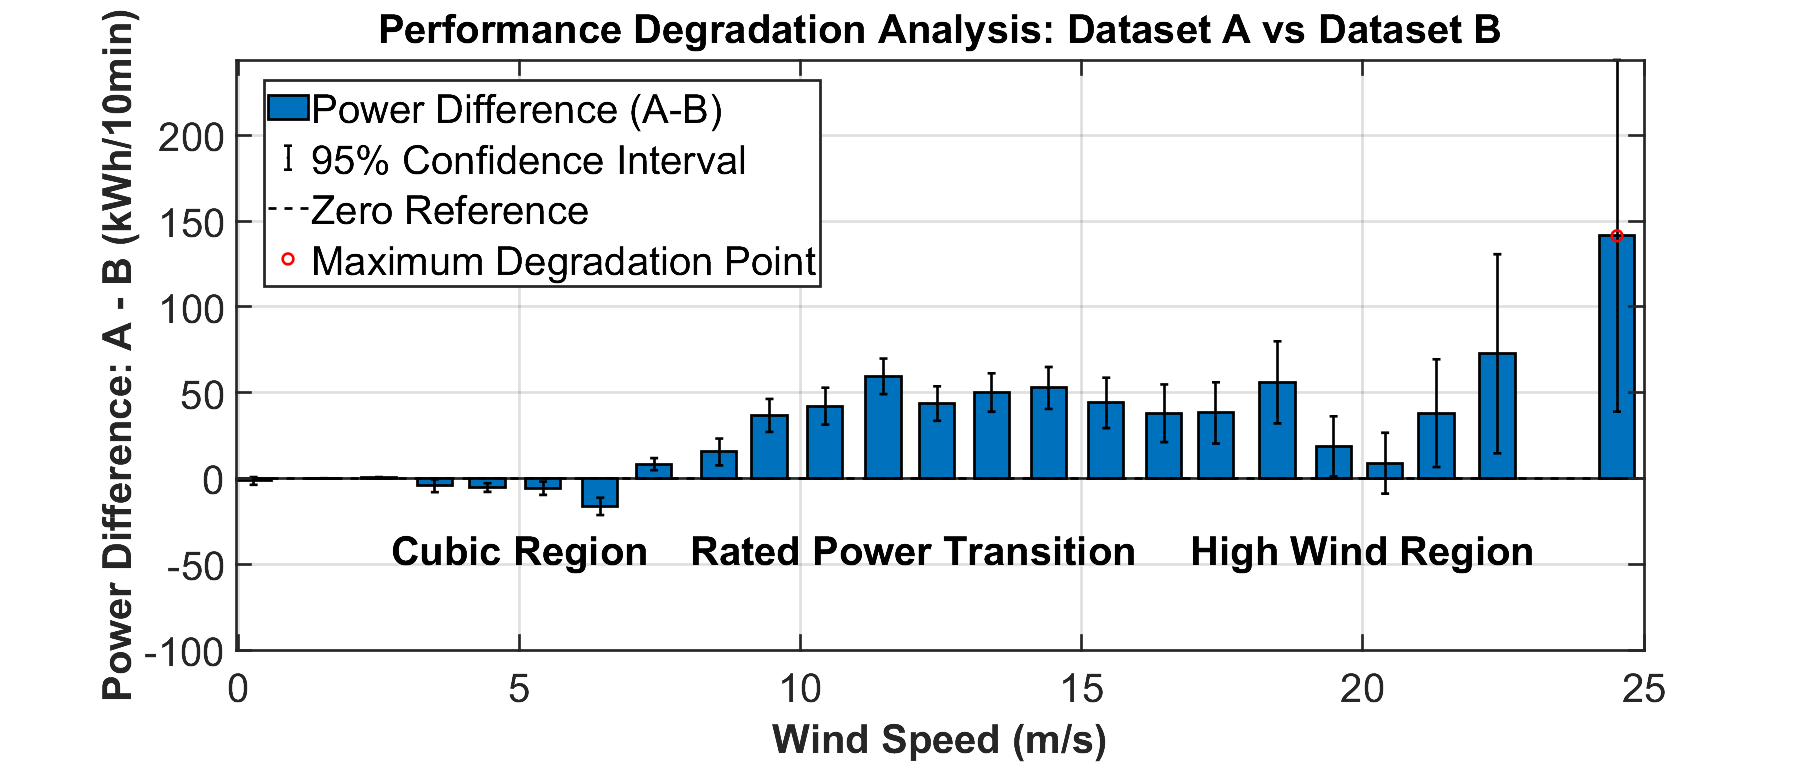
\includegraphics[width=\textwidth]{Figure3_PerformanceDegradation.png}
    \caption{Performance Degradation Analysis comparing Datasets A and B across wind speed bins.}
    \label{fig:performance_degradation}
\end{figure}
% First table - placed at document level

\vspace{-20pt}

\subsection*{Working Hypothesis: Pitch System Faults and Yaw Misalignment}
As shown in the figure \ref{fig:performance_degradation}, the presence of slight negative difference values in the 4-6 m/s range of the cubic region suggests Dataset B actually outperforms Dataset A at very low wind speeds. This counterintuitive finding could indicate a control system recalibration that prioritised low-wind performance at the expense of high-wind operation. The  figure \ref{fig:performance_degradation} shows a distinctive step-change in performance at 8 m/s, which might be the typical point where blade pitch control transitions from maximum power extraction to power regulation mode. This might suggests pitch control system miscalibration rather than mechanical wear as a primary cause. Furthermore, Blade pitch control system misalignment or malfunction, Yaw system directional errors could reduce effective wind capture, and Grid connectivity disturbances could also trigger protective derating, along with Possible mechanical component degradation (bearings, gearbox). According to blade element momentum theory, pitch errors alter the blade's angle of attack, reducing the lift coefficient across the blade span, demonstrates that even small pitch angle errors in the below-rated region cause significant power production losses. The pattern of degradation seen in Dataset B, particularly in the cubic region of the power curve, corresponds with documented cases of pitch system miscalibration, where the performance impact is most pronounced at moderate wind speeds before rated power is achieved. The power reduction pattern across different wind speed bins further supports this conclusion, as yaw misalignment effects become more pronounced at higher wind speeds where maximum energy capture depends on precise rotor positioning. 

 
 

 \newpage
\section*{ Bayesian Analysis of Binary Symmetric Channel Performance}
\subsection*{Theory and Decision Framework}
\label{sec:theory}



In communications engineering, the Binary Symmetric Channel (BSC) helps making optimal decisions about transmitted data with noise, where Bayesian inference derive statistically optimal detection rules based on both channel characteristics and prior knowledge, updating probability estimates when new evidence becomes available as Posterior = (Likelihood × Prior) / Evidence and based on Bayes' theorem and the denominator can be expanded using the law of total probability:
 
\begin{equation}
P(B_i|A_j) =\frac{P(A_j|B_i)P(B_i)}{\sum_k P(A_j|B_k)P(B_k)}
=\frac{P(A_j|B_i)P(B_i)}{P(A_j|B_1)P(B_1) + P(A_j|B_2)P(B_2)}
\end{equation}
 

% Enhanced BSC State Transition Summary Table with Key Equations
\begin{table}[htb]
\centering
\caption{Binary Symmetric Channel: Transition Probabilities and Key Equations}
\renewcommand{\arraystretch}{1.7}
\begin{tabular}{@{}p{0.27\textwidth}p{0.35\textwidth}p{0.36\textwidth}@{}}
\toprule
\textbf{Component} & \textbf{Mathematical Expression} & \textbf{Description} \\
\midrule
\multicolumn{3}{@{}l}{\textbf{Transmission States}} \\
Prior probabilities & $P(B_1) = p$ \newline $P(B_2) = 1-p$ & Probability of sending bit ``0'' \newline Probability of sending bit ``1'' \\
\midrule
\multicolumn{3}{@{}l}{\textbf{Channel Characteristics}} \\
Correct transmission & $P(A_1|B_1) = P(A_2|B_2) = q$ & Probability bit arrives unchanged \\
Error transmission & $P(A_2|B_1) = P(A_1|B_2) = 1-q$ & Probability bit is flipped \\
\midrule
\multicolumn{3}{@{}l}{\textbf{Receiver Probabilities}} \\
Probability of receiving ``0'' & $P(A_1) = qp + (1-q)(1-p)$ & Total probability of bit ``0'' reception \\
Probability of receiving ``1'' & $P(A_2) = (1-q)p + q(1-p)$ & Total probability of bit ``1'' reception \\
\midrule
\multicolumn{3}{@{}l}{\textbf{Bayesian Posterior Probabilities}} \\
Given received ``0'' & $P(B_1|A_1) = \frac{qp}{qp + (1-q)(1-p)}$ \newline $P(B_2|A_1) = \frac{(1-q)(1-p)}{qp + (1-q)(1-p)}$ & Probability ``0'' was transmitted \newline Probability ``1'' was transmitted \\
Given received ``1'' & $P(B_1|A_2) = \frac{(1-q)p}{(1-q)p + q(1-p)}$ \newline $P(B_2|A_2) = \frac{q(1-p)}{(1-q)p + q(1-p)}$ & Probability ``0'' was transmitted \newline Probability ``1'' was transmitted \\
\midrule
\multicolumn{3}{@{}l}{\textbf{MAP Decision Boundaries for Case 2}} \\
When receiving ``0'' & $P(B_1|A_1) = P(B_2|A_1) \Rightarrow p = 1-q$ & Decision threshold for bit ``0'' \\
When receiving ``1'' & $P(B_1|A_2) = P(B_2|A_2) \Rightarrow p = q$ & Decision threshold for bit ``1'' \\
\bottomrule
\label{calculation}
\end{tabular}
\end{table}

\vspace{-60pt}

\subsubsection*{Case 1: Analysis of Receiver Probabilities explained by $P(A_1) = qp + (1-q)(1-p)$}
\vspace{-5pt}
Shown in figure \ref{fig:case1}, when $p=0.5$ (red line), $P[A_1]$ remains constant at $0.5$ regardless of channel quality $q$. This represents the unbiased case where both bits are equally likely to be transmitted. For $p=0.7$ (green line), $P[A_1]$ increases with $q$, while for $p=0.3$ (blue line), $P[A_1]$ decreases with $q$. This shows that when $q>0.5$, the channel tends to preserve the transmitter's bit distribution. When $q=0.7$, $P[A_1]$ increases with $p$, while when $q=0.3$, $P[A_1]$ decreases with $p$. This demonstrates that channel quality determines whether the received bit distribution follows or inverts the transmitted distribution. All curves intersect at $q=0.5$, indicating that when the channel is purely random, the prior probabilities have no effect on reception statistics.  The derivative $\frac{\partial P(A_1)}{\partial p} = 2q-1$ is positive when $q>0.5$ and negative when $q<0.5$, explaining the slope directions in the plots.
 

   
 

% Case 1: Receiver Probabilities Analysis
\begin{figure}[H]
    \centering
    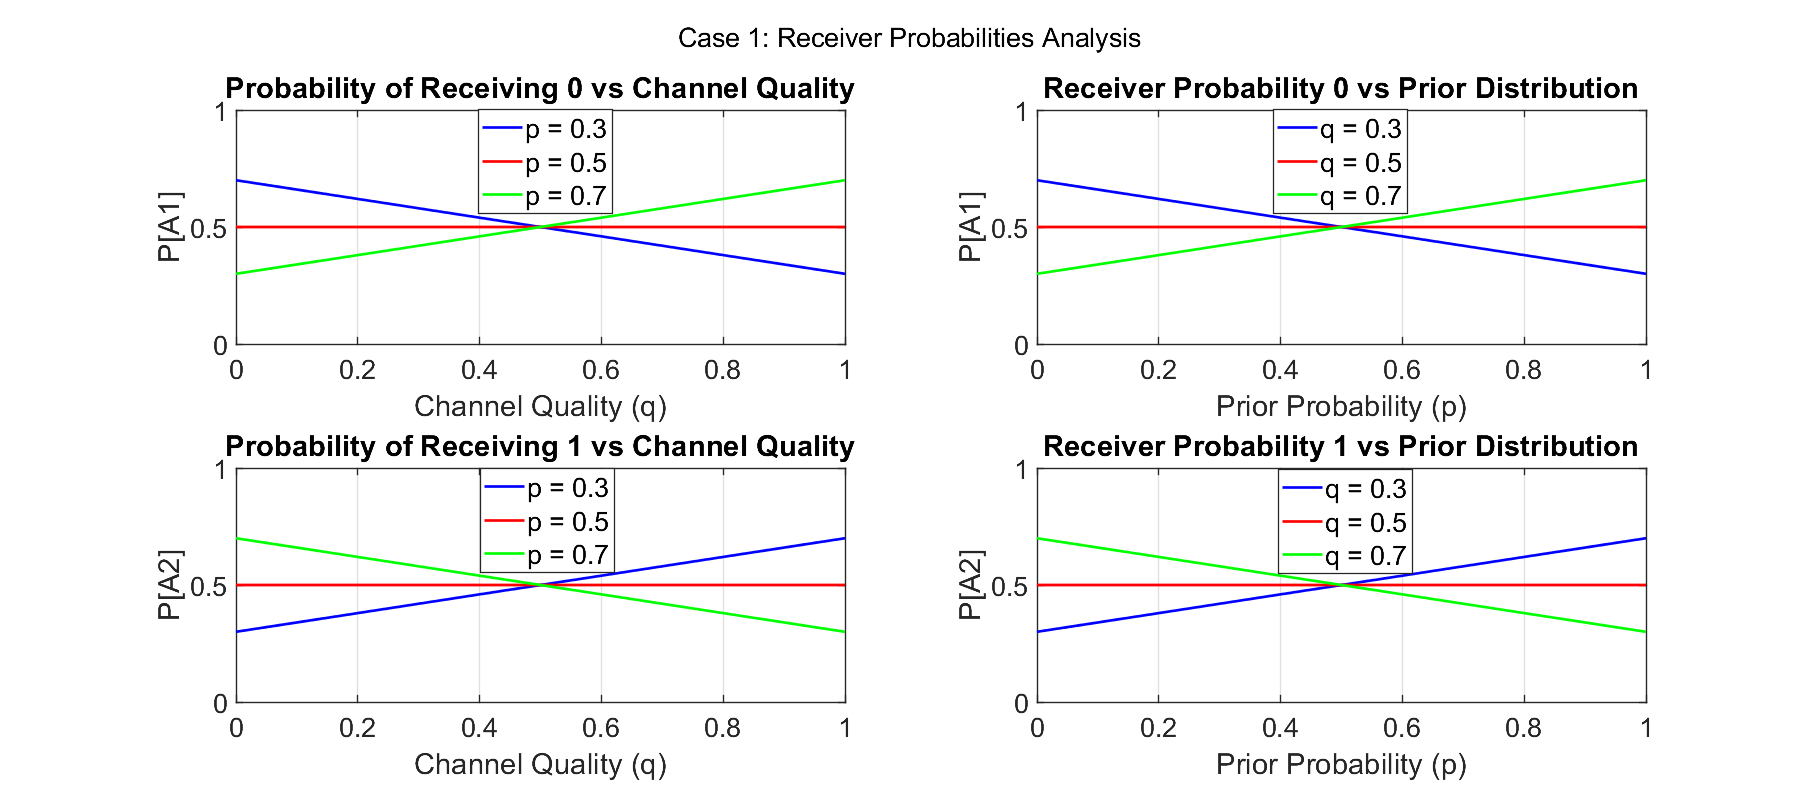
\includegraphics[width=\textwidth]{photo/BSC_Analysis_Case1.png}
    \caption{Case 1: Receiver Probabilities Analysis showing probability of receiving bit ``0'' and bit ``1'' as functions of channel quality ($q$) and prior probability ($p$).}
    \label{fig:case1}
\end{figure}
\vspace{-10pt}
Revealed in figure \ref{fig:case1}, these mathematical relationships support several critical engineering applications: real-time channel quality estimation through reference sequence comparison, adaptive modulation schemes that implement higher-order modulations (64-QAM, 256-QAM) when \( q > 0.7 \) and robust BPSK with stronger coding when \( q < 0.5 \), and power optimisation for energy-constrained IoT devices—conserving energy in regions where marginal power increases yield minimal reception improvements. The critical threshold at \( q = 0.5 \) serves as a fundamental decision point for adaptive systems, informing the design of receiver circuits that automatically adjust to changing channel characteristics. Additionally, the \( P[A_1] \) vs \( p \) curves with varying \( q \) values enable tailored error correction strategies, employing minimal redundancy codes for reliable channels (\( q \approx 0.7 \)) and progressively stronger coding schemes as channel quality deteriorates.
% Case 2: MAP Decision Boundaries
\begin{figure}[H]
    \centering
    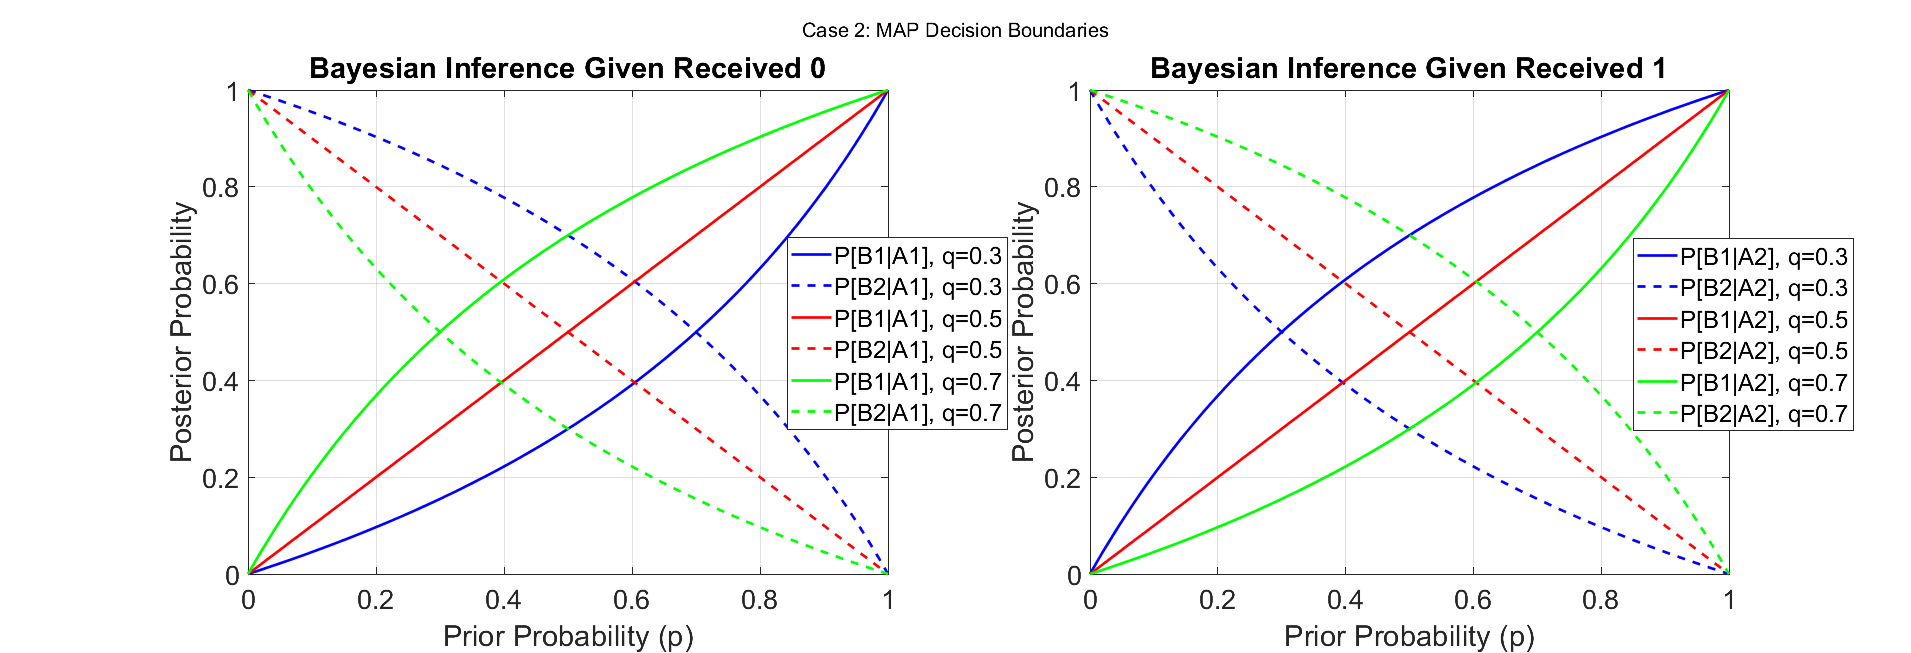
\includegraphics[width=\textwidth]{photo/BSC_Analysis_Case2.png}
    \caption{Case 2: MAP Decision Boundaries showing posterior probabilities $P[B_1|A_1]$, $P[B_2|A_1]$, $P[B_1|A_2]$, and $P[B_2|A_2]$ as functions of prior probability ($p$) for different channel quality values ($q$).}
    \label{fig:case2}
\end{figure}
\vspace{-10pt}
Figure \ref{fig:case2} reveal optimal Bayesian decision boundaries for receiver design based on Maximum A Posteriori (MAP) principles. When receiving bit "0" ($A_{1}$), the plots demonstrate that the critical decision threshold occurs precisely at $p = 1 - q$, with $P[B_{1}|A_{1}] > P[B_{2}|A_{1}]$ when $p > 1 - q$, indicating the receiver should decide bit "0" was transmitted. Conversely, when receiving bit "1" ($A_{2}$), the decision threshold occurs at $p = q$, with $P[B_{2}|A_{2}] > P[B_{1}|A_{2}]$ when $p < q$, indicating the receiver should decide bit "1" was transmitted. As the channel reliability improves (e.g., $q > 0.7$), the decision regions become increasingly asymmetric, allowing more aggressive bias towards the more reliable information source. At $q = 0.5$ (purely random channel), the MAP decision relies solely on prior probabilities, defaulting to the more likely transmitted bit. For channels with $q < 0.5$ (bit-inverting behaviour), the receiver counterintuitively decides the opposite of what intuition might suggest—choosing transmitted "1" when receiving "0" if $p < 0.5$. These MAP decision boundaries directly inform practical soft-decision decoders, adaptive threshold circuits, and dynamic error correction strategies that optimise reception reliability whilst minimising computational complexity in modern communication systems.
 



\end{document}
